%% ------- ROZDZIAŁ 3 ------- %%

\chapter{Przedstawienie aplikacji}
Na potrzeby tej pracy została napisana aplikacja w języku programowania Python w wersji 2.7, która ma za zadanie przedstawić część możliwości pakietu \textit{Scikit-learn} analizując dane giełdowe.
Zastosowany został graficzny interfejs użytkownika (GUI), dzięki któremu jest możliwa szybka zmiana wybranych opcji, oraz dokonywanie wielu analiz bez potrzeby ponownego uruchamiania aplikacji.
Przeznaczeniem aplikacji jest analiza danych, tak więc generowane wyniki zapisywane są we wskazanym przez użytkownika katalogu, a także wyświetlane bezpośrednio w aplikacji.

\section{Podstawowe założenia}
Aplikacja została napisana w modelu orientowanym obiektowo. Starano się zachować wyraźny podział na część biznesową, oraz interfejs użytkownika. W związku z tym struktura katalogów w projekcie wygląda następująco:
\dirtree{%
.1 /. 
.2 /mdata.
.3 /client.
.3 /drivers. 
.4 /config.
.4 /databases.
.3 /gui. 
.4 /buttons.
.4 /items.
.4 /layouts.
.4 /screens.
}

W katalogu \textit{/client} umieszczony został kod odpowiadający za pobieranie danych giełdowych, przeprowadzanie analizy regresji, oraz generowanie wykresów.
Katalog \textit{/drivers} zawiera mechanizmy zapisu i odczytu głównego pliku konfiguracyjnego aplikacji, oraz mechanizm bazodanowy napisany przy pomocy pakietu \textit{SqlAlchemy}.
Ostatni katalog \textit{/gui} zawiera wszystkie elementy graficznego interfejsu użytkownika, w podziale na przyciski, układy, okna oraz pozostałe elementy.\\

Przeprowadzono analizę kodu dla katalogu \textit{/mdata} programem \textit{pylint}.\\
Według tego raportu kod aplikacji uzyskał ocenę 7.28/10 i zawiera:
\begin{itemize}
 \item 43 zaimplementowane klasy
 \item 199 zaimplementowanych metod
 \item 2 funkcje pozaklasowe
 \item 1707 linii kodu
\end{itemize}


\subsection{Dane giełdowe}

Ze względu na ogromne możliwości pakietu \textit{Scikit-learn}, a także na ograniczenia dotyczące samej konstrukcji aplikacji, poczynione zostały pewne założenia definiujące działanie aplikacji.\\

Główne założenia związane z pobieraniem danych giełdowych:
\begin{itemize}
 \item Dane giełdowe pobierane są na podstawie wcześniej przygotowanej bazy firm giełdy amerykańskiej
 \item Pobieranie danych giełdowych odbywa się za pomocą API \textit{Yahoo Finance}
 \item Rodzaj danych jest determinowany jedynie przez użyte API, a ich zakres wybierany jest poprzez podanie daty początkowej i końcowej\\
\end{itemize}

Zastosowane w pracy API \textit{Yahoo Finance} umożliwia pobieranie danych jedynie w jednej postaci, bez możliwości wyboru lub dodania dodatkowych elementów.
Każde pobranie danych w tym samym zakresie powoduje otrzymanie dokładnie takich samych rezultatów, co kwalifikuje to API do udziału w analizie.
Do bezpośredniego pobierania danych zastosowano funkcję \textit{DataReader} pakietu \textit{pandas\_datareader}.
Umożliwia ona prostą implementację API w języku Python oraz zwracanie danych w pożądanym formacie \textit{pandas.DataFrame}.\\

Dane zwracane przez API dzielą się na:
\begin{itemize}
 \item \textit{Open}: cena początkowa (otwarcia)
 \item \textit{Close}: cena końcowa (zamknięcia) 
 \item \textit{High}: najwyższa wartość ceny 
 \item \textit{Low}: najniższa wartość ceny 
 \item \textit{Adj Close}: skorygowana wartość ceny końcowej
 \item \textit{Volume}: wartość wolumenu
\end{itemize}

\newpage

Przykładowe zastosowanie funkcji \textit{DataReader} do pobierania danych giełdowych za pomocą API \textit{Yahoo Finance}:

\begin{lstlisting}
 >>> from pandas_datareader.data import DataReader
 >>> source = 'yahoo'
 >>> company = 'AAPL'
 >>> start = '2017-12-01'
 >>> end = '2017-12-02'
 >>> DataReader(company, source, start, end)
                   Open        High         Low \      
 Date
 2017-12-01  170.429993  172.139999  168.440002  
 2017-12-02  169.949997  171.669998  168.500000  
 
                  Close   Adj Close     Volume
 Date
 2017-12-01  171.850006  171.850006   41527200
 2017-12-02  171.050003  171.050003   39759300
>>>
\end{lstlisting}

\subsection{Analiza danych giełdowych}

Główne założenia związane z analizą danych:
\begin{itemize}
 \item Do analizy można wykorzystać dane jednego, wskazanego przez użytkownika rodzaju (Open, Close, High, Low)
 \item Analiza danych może być przeprowadzona jedną z czterech zaimplementowanych metod regresji z pakietu \textit{Scikit-learn}
 \item Podział danych na zbiór danych uczących i zbiór danych testowych następuje poprzez wybranie wartości procentowej ilości danych uczących w oknie opcji aplikacji
\end{itemize}

Ograniczenie rodzaju analizowanych danych umożliwia zawężenie czynników, które mogą wpłynąć na wyniki badań, co prowadzi do poprawy wiarygodności otrzymanych rezultatów.
Z drugiej jednak strony, może to prowadzić do otrzymania wyników różniących się od tych, które byłyby otrzymywane z pełnego zbioru danych.\\

Do przeprowadzenia badań wybrano i wykorzystano jedną metodę analizy regresji liniowej, oraz trzy metody analizy regresji nieliniowych dostępne w pakiecie \textit{Scikit-learn}.
Są to:
\begin{itemize}
 \item Regresja liniowa
 \item Regresja Grzbietowa
 \item Regresja Wektorów Nośnych (SVR)
 \item Regresja Procesu Gaussa (GPR)
\end{itemize}

Przeprowadzone analizy skupiają się na róznicach pomiędzy zdolnościami predykcyjnymi wyżej wymienionych metod regresji oraz ich zdolnościach do opisywania trendów dla danego zakresu danych.
Opisana została także różnica w dokładności metod regresji w zależności od proporcji ilości danych uczących i testowych.


\section{Zastosowane pakiety języka Python}

\subsection{Kivy}
\textit{Kivy} jest biblioteką języka programowania Python umożliwiającą tworzenie graficznego interfejsu użytkownika przeznaczonego na wiele platform, takich jak Windows, Linux, iOS czy Android.
Jego główną zaletą jest możliwość oddzielenia warstwy biznesowej aplikacji od warstwy prezentacji, co wpływa zarówno na czytelność, skalowalność i ogólną jakość kodu.\\

Są możliwe dwa warianty budowania aplikacji za pomocą tego pakietu. Pierwszy umożliwia tworzenie plików w języku \textit{Kivy Design Language}, które definiują wygląd aplikacji.
Pliki te są następnie importowane do kodu w języku Python, a na ich podstawie generowane jest GUI.\\

Drugi wariant polega na użyciu odpowiednich klas udostępnianych przez pakiet bezpośrednio kodzie języka Python. Ze względu na lepszą organizację kodu, w niniejszej pracy zastosowano wariant drugi.\\

Podstawowym podziałem okien w pakiecie \textit{Kivy} są okna i układy.
Okna pozwalają na tworzenie wielu niezależnych od siebie kart i zakładek. Żeby umożliwić wstawienie jakiegokolwiek elementu funkcjonalnego do danego okna, należy najpierw "nałożyć na niego" jeden lub kilka układów.
W taki sposób można dzielić odpowiednie okna na części, na przykład tworząc "menu".\\

W niniejszej pracy zastosowano wzorzec polegający na tworzeniu i umieszczaniu każdego elementu GUI w osobnej klasie, oraz osobnym pliku \textit{.py}. Umożliwia to większą kontrolę nad poszczególnymi elementami, a także zwiększa skalowalność.\\
Przykładowy kod prezentujący implementację przycisku wyboru okna analizy regresji:
\begin{lstlisting}
 from kivy.uix.button import Button


 class RegressionButton(Button):
     def __init__(self, base, **kwargs):
         self.base = base
         self.text = 'Regression\n  Analysis'
         super(RegressionButton, self).__init__(**kwargs)
 
     def on_press(self):
         if not self.base.screen_manager.current\
                 == self.base.screens['regression'].name:
             self.base.screen_manager.switch_to(
			    self.base.screens['regression'])
\end{lstlisting}


\subsection{Pandas i Matplotlib}
Biblioteka \textit{Pandas} udostępnia bardzo rozbudowane narzędzia do przechowywania i analizy danych.
W niniejszej pracy wykorzystano należącą do niej klasę \textit{DataFrame} w celu przechowywania danych giełdowych pobranych za pomocą funkcji \textit{DataReader}, oraz przygotowywania tych danych do wygenerowania wykresów.\\

Większość elementów biblioteki \textit{Pandas} wykorzystuje możliwości pakietów takich jak \textit{NumPy} i \textit{SciPy} jako bazę, tak więc są one w pełni kompatybilne z obiektami tychże pakietów.
Głównym elementem wykorzystanym w pracy jest obiekt \textit{DataFrame}, który jest kontenerem zarówno dla oryginalnych pobranych danych giełdowych, jak i dla wyników analizy regresji.\\
Przykładowo, po dokonanej analizy regresji budowany jest obiekt:
\begin{lstlisting}
 df_all_results = pd.DataFrame(
            index=all_dates,
            data={chosen_data_type: all_values,
                  'Regression': sort_pred})
\end{lstlisting}

Przyjmuje on jako argumenty:
\begin{itemize}
 \item \textit{index}: obiekt typu \textit{numpy.ndarray} zawierający listę dat dla osi X wykresu
 \item \textit{data}: słownik zawierający oryginalne dane, oraz wyniki predykcji, także typu \textit{numpy.ndarray}
\end{itemize}

Biblioteka \textit{Pandas} jest także w pełni kompatybilna z biblioteką \textit{Matplotlib}, która umożliwia generowanie wykresów na podstawie podanych danych.
W pracy zastosowano metodę \textit{plot()} udostępnianą przez obiekt \textit{DataFrame}, która zwraca gotowy obiekt klasy \textit{matplotlib.axes.Axes}.
Obiekt ten, uzupełniony o niezbędne elementy i parametry, jest gotowy do wyświetlenia lub zapisania wykresu na dysku, poprzez "wyciągnięcie" figury metodą \textit{get\_figure()} i zastosowania na niej metody \textit{savefig()}.\\

Przykładowy kod generowania wykresu wyników analizy regresji, z dodaniem pionowej linii oznaczającej podział danych na uczące i testowe:
\begin{lstlisting}
 df_reg_results = self.reg_data['df_all_results']
 
 self.regression_plot = df_reg_results.plot(title=plot_title,
				            grid=True)
 self.regression_plot.axvline(x=self.reg_data['train_test_v_date'],
                              color='red')
 self.regression_plot.set_ylabel('Price')
 self.regression_plot.set_xlabel('Date')
 
 self.regression_fig = self.regression_plot.get_figure()
 
 self.regression_fig.savefig('{dir}\{file}'\
                             .format(dir=self._get_tempdir(),
				     file=self.diagram_names['reg']))
\end{lstlisting}

\subsection{Scikit-learn}
Biblioteka \textit{Scikit-learn} i jej możliwości jest głównym tematem niniejszej pracy. W aplikacji zaimplementowano cztery rodzaje analizy regresji: regresję liniową, grzbietową, wektorów nośnych i procesu Gaussa.\\

Przygotowanie danych do analizy dla wszystkich metod jest identyczne:
\begin{lstlisting}
 data = deepcopy(self.data)
 split_rate = self.get_split_rate()
 chosen_data_type = self.get_data_type()
 all_data_types = self.regression_data_types
 data_to_drop = [data_t for data_t in all_data_types
                 if data_t != chosen_data_type]

 sort = data.drop(data_to_drop, axis=1)
 sort_values = np.concatenate(sort.values)
 sort_dates = sort.index.values

 original_dates, dates_delta = self.change_dates(sort_dates)
 dates_delta = np.reshape(dates_delta, (len(dates_delta), 1))

 sc_x = StandardScaler()
 sc_y = StandardScaler()

 sort_dates = sc_x.fit_transform(dates_delta)
 sort_values = sc_y.fit_transform(sort_values)

 sort_dates_train, sort_dates_test = self.split_data(sort_dates,
                                                     split_rate)
 sort_values_train, sort_values_test = self.split_data(sort_values,
                                                       split_rate)
\end{lstlisting}

W pierwszej kolejności pobrane dane zawierające wszystkie kolumny z cenami walut wolumenem są redukowane do jedjen wybranej wcześniej kolumny.
Tak przygotowane dane dzielone są na ceny i daty i przechowywane w obiektach typu \textit{numpy.ndarray}, odpowiednio: \textit{sort\_values} i \textit{sort\_dates}.
Daty konwertowane są na wartości typu \textit{Integer} przedstawiające odległość danej daty od pierwszej podanej na potrzeby późniejszej analizy regresji. Przekształcana jest również macierz dat z jednowymiarowej na dwuwymiarową.\\

Kolejnym krokiem jest użycie obiektu klasy \textit{sklearn.preprocessing.StandardScaler} w celu przeprowadzenia normalizacji danych.
Obiekt ten udostępnia metody \textit{fit\_transform()} oraz \textit{inverse\_transform()}, które pozwalają na odpowiednio: przeprowadzenie normalizacji danych oraz powrót do oryginalnych wartości.\\

Tak przygotowane dane są następnie dzielone na zbiory uczące i testowe za pomocą osobnej metody.\\

Obiekt klasy \textit{sklearn.linear\_model.LinearRegression} został użyty do przeprowadzenia regresji liniowej:
\begin{lstlisting}
 linear_reg = LinearRegression(fit_intercept=False)
 linear_reg.fit(sort_dates_train, sort_values_train)
 sort_pred = linear_reg.predict(sort_dates)
\end{lstlisting}
Pierwszym krokiem jest stworzenie obiektu \textit{linear\_reg}, podając jako argument \textit{fit\_intercept=False}.
Tak przygotowany obiekt udostępnia metodę \textit{fit()}, której argumentami są zbiory danych uczących, odpowiednio dat i cen akcji.
Metoda ta przygotowuje model do predykcji, którą wykonuje się za pomocą kolejnej metody \textit{predict()}, jako argumenty podając zbiór wszystkich dat, zarówno testowych jak i uczących.
Pozwala to na stworzenie prostej regresji dla całego zbioru danych.\\

Klasa \textit{sklearn.kernel\_ridge.KernelRidge} pozwala na przeprowadzenie analizy regresji grzbietowej która, zaliczając się do regresji nieliniowych, została wzbogacona o obiekt klasy \textit{sklearn.model\_selection.GridSearchCV}:
\begin{lstlisting}
 krr = GridSearchCV(
         KernelRidge(kernel='rbf'),
                     param_grid={"alpha": [1e0, 0.1, 1e-2, 1e-3],
                                 "gamma": np.logspace(-2, 2, 5)})

 krr.fit(sort_dates_train, sort_values_train)
 sort_pred = krr.predict(sort_dates)
\end{lstlisting}

Obiekt \textit{KernelRidge} przyjmuje parametry \textit{alpha} i \textit{gamma}, których dopasowanie jest niezmierne istotne przy przeprowadzaniu poprawnej analizy.
Znalezienie poprawnego dopasowania parametrów jest znacznie uproszczone w przypadku wykorzystania obiektu \textit{GridSearchCV}, 
który dla podanego obiektu regresji i parametrów określonych w \textit{param\_grid} automatycznie dopasowuje najlepsze parametry.
Tworzy on iloczyn kartezjański wszystkich podanych argumentów, i podczas działania kolejnego kroku, czyli metody \textit{fit()} wybiera taki zbiór, który jest najlepiej dopasowany.\\

W przypadku pozostałych metod regresji, czyli Regresji Wektorów Nośnych i Regresji Procesu Gaussa zastosowano ten sam mechanizm dobierania parametrów obiektu.
Pierwsza z nich udostępniona jest przez obiekt klasy \textit{sklearn.svm.SVR}, a druga przez obiekt klasy \textit{sklearn.gaussian\_process.GaussianProcessRegressor}.


\section{Opis funkcjonalności aplikacji}
Aplikacja została napisana w języku programowania Python w środowisku Windows 10 Home.
Do poprawnego uruchomienia wymaga zainstalowanego interpretera języka Python w wersji 2.7, oraz zainstalowanych bibliotek zewnętrznych, z których najważniejsze to:
\begin{itemize}
 \item Matplotlib, Pandas, Numpy i SciPy
 \item Scikit-learn
 \item Kivy
 \item Pandas\_datareader
 \item Configparser
 \item SqlAlchemy
\end{itemize}

Wszystkie biblioteki użyte w pracy dostępne są na licencjach open-source i są gotowe do pobrania poprzez interfejs \textit{PyPa - Python Package Index}.\\

Aplikacja podzielona jest na trzy okna:
\begin{itemize}
 \item Okno instrukcji
 \item Okno opcji
 \item Okno analizy regresji
\end{itemize}

Po uruchomieniu aplikacji użytkownikowi jako pierwsze przedstawiane jest okno instrukcji, które zawiera schemat kroków potrzebnych do poprawnego przeprowadzenia analizy.
\begin{figure}[ht]
\centering
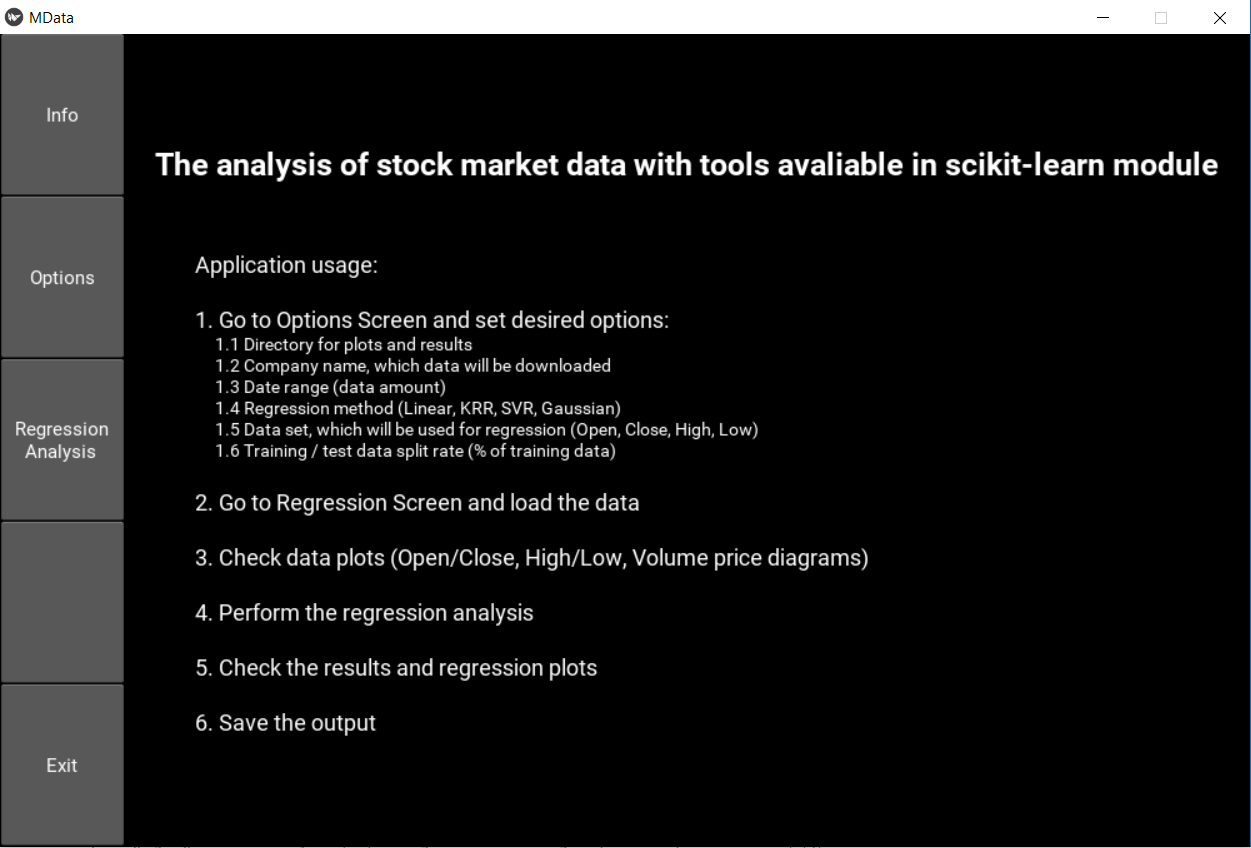
\includegraphics[scale=0.4]{pictures/app_info_screen.png}
\caption{Aplikacja: okno instrukcji}
\label{fig:app_instrukcja}
\end{figure}

Z lewej strony dostępny jest pasek menu, który zawiera przyciski: \textit{Info}, \textit{Options}, \textit{Regression analysis} oraz \textit{Exit}.
Każdy z nich pozwala na wyświetlenie innego okna aplikacji, z wyjątkiem przycisku \textit{Exit} który wywołuje okno z zapytaniem o zakończenie pracy programu.

\subsection{Okno opcji}
W oknie opcji użytkownik może zmienić lub ustawić parametry, które będą używane w późniejszej analizie regresji.

\newpage

\begin{figure}[ht]
\centering
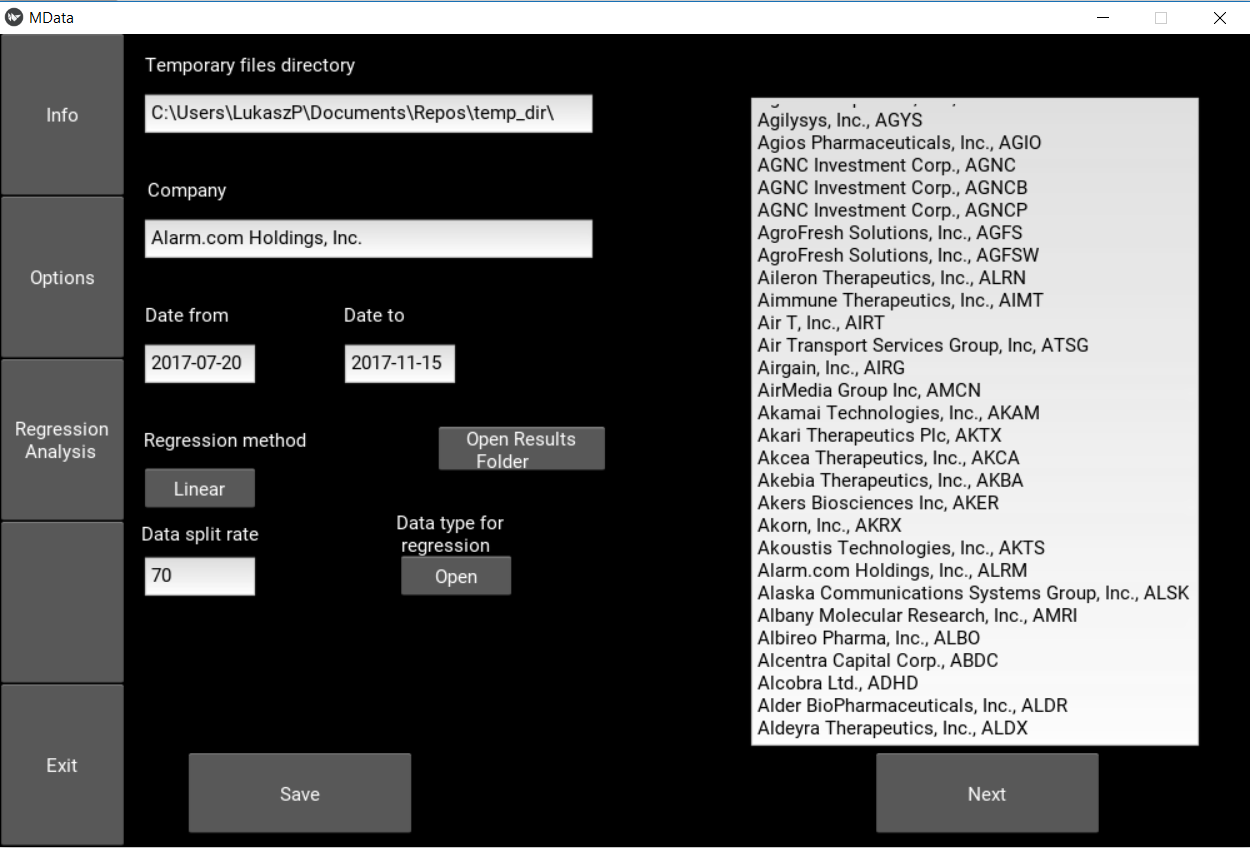
\includegraphics[scale=0.4]{pictures/app_options_screen.png}
\caption{Aplikacja: okno opcji}
\label{fig:app_okno_opcji}
\end{figure}

Parametry możliwe do zmiany to:
\begin{itemize}
 \item \textit{Temporary files directory}: ścieżka do folderu, do którego mają być zapisywane wyniki
 \item \textit{Company}: nazwa firmy, dla której mają być pobrane dane
 \item \textit{Date from}: data od której mają być pobrane dane, w formacie yyyy-mm-dd
 \item \textit{Date to}: data do której mają być pobierane dane, w formacie yyyy-mm-dd
 \item \textit{Regression method}: lista typu dropdown z możliwością wyboru metody regresji
 \item \textit{Data split rate}: wartość procentowa ilości danych uczących względem danych testowych
 \item \textit{Data type for regression}: lista typu dropdown umożliwiająca wybór typu danych do analizy
\end{itemize}

Do zapisania konfiguracji służy przycisk \textit{Save} który, ze względu na walidację każdego pola lub listy, po wciśnięciu poinformuje użytkownika o powodzeniu lub niepowodzeniu operacji.
W przypadku niepowodzenia użytkownikowi zostaje wskazane pole, które zostało źle wypełnione.\\

Lista firm, dla których jest możliwość pobrania danych znajduje się w zablokowanym polu tekstowym z prawej strony okna.
Jako, iż istnieje możliwość kopiowania tekstu z tego pola, aby wypełnić parametr \textit{Company} należy skopiować dokładną nazwę firmy i wkleić ją we właściwe miejsce.
Przycisk \textit{Next} pozwala natomiast na wyświetlenie kolejnej części listy firm, która jest posortowana alfabetycznie.

\subsection{Okno analizy regresji}
W oknie analizy regresji użytkownik może przeprowadzić operacje: pobrania danch giełdowych i przeprowadzenia analizy, zgodnie z parametrami ustawionymi w oknie opcji.

\newpage

\begin{figure}[ht]
\centering
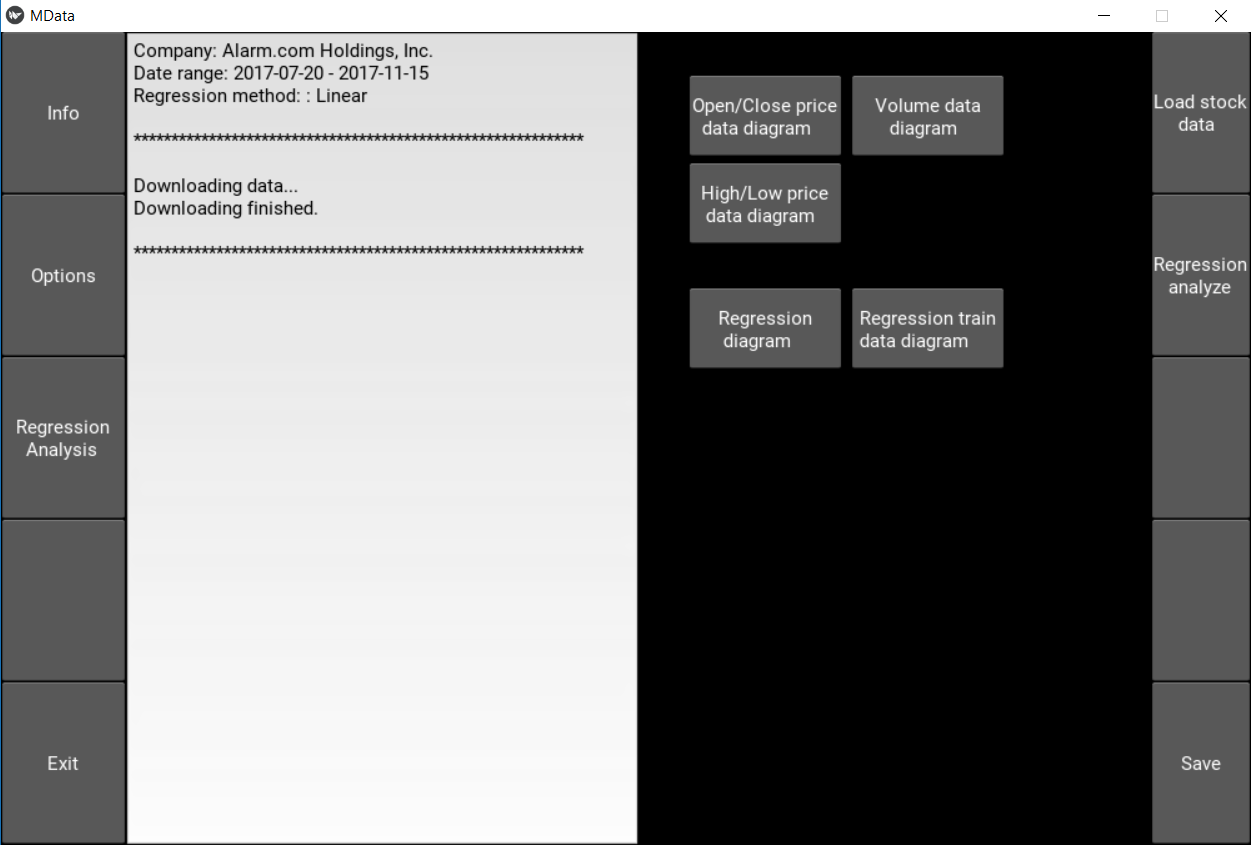
\includegraphics[scale=0.4]{pictures/app_reg_screen_data_loaded.png}
\caption{Aplikacja: okno analizy regresji (pobrane dane giełdowe)}
\label{fig:app_okno_reg}
\end{figure}

Z prawej strony okna znajduje się pasek menu z przyciskami: \textit{Load stock data}, \textit{Regression analyze} oraz \textit{Save}.
Z lewej strony znajduje się natomiast zablokowane pole tekstowe, w którym pojawiają się wyniki i informacje.
W centralnej części obecne są przyciski, które są odpowiedzialne za wyświetlanie odpowiednich wykresów:
\begin{itemize}
 \item \textit{Open/Close price data diagram}
 \item \textit{High/Low price data diagram}
 \item \textit{Volume data diagram}
 \item \textit{Regression diagram}
 \item \textit{Regression train data diagram}
\end{itemize}

\begin{figure}[ht]
\centering
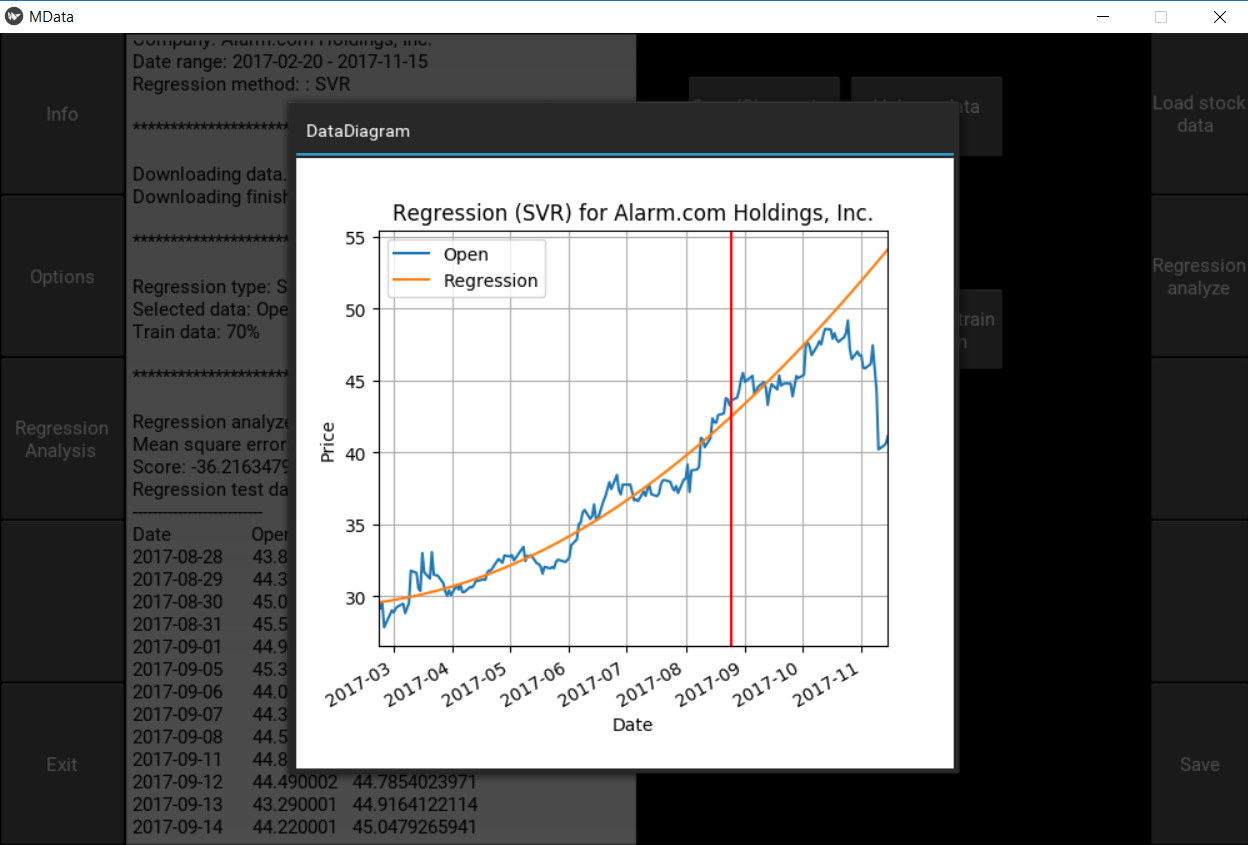
\includegraphics[scale=0.4]{pictures/app_reg_screen_plot.png}
\caption{Aplikacja: Wykres rezultatu analizy regresji}
\label{fig:app_regresja}
\end{figure}

Pierwsze trzy wykresy przedstawiają niemodyfikowane dane giełdowe pobrane za pomocą przycisku \textit{Load stock data} i tylko po jego wciśnięciu będą dostępne.
Ostatnie dwa wykresy udostępnione zostają po przeprowadzeniu analizy regresji i przedstawiają odpowiednio: rezultat analizy regresji dla całości danych oraz rezultat zawężony jedynie do danych testowych.

\section{diagramy UML}
Ze względu na dużą ilość klas, w szczególności należących do graficznego interfejsu użytkownika, przedstawienie pełnego diagramu klasowego UML nie jest możliwe.
Wyróżnić można natomiast trzy główne funkcje aplikacji, które przedstawione na diagramie UML mogą posłużyć jako dobre odzwierciedlenie działania aplikacji.

\subsection{Zapis parametrów w oknie opcji}
Pierwszą główną funkcją aplikacji jest zapis wybranych przez użytkownika parametrów do pliku konfiguracyjnego.\\
\begin{figure}[ht]
\centering
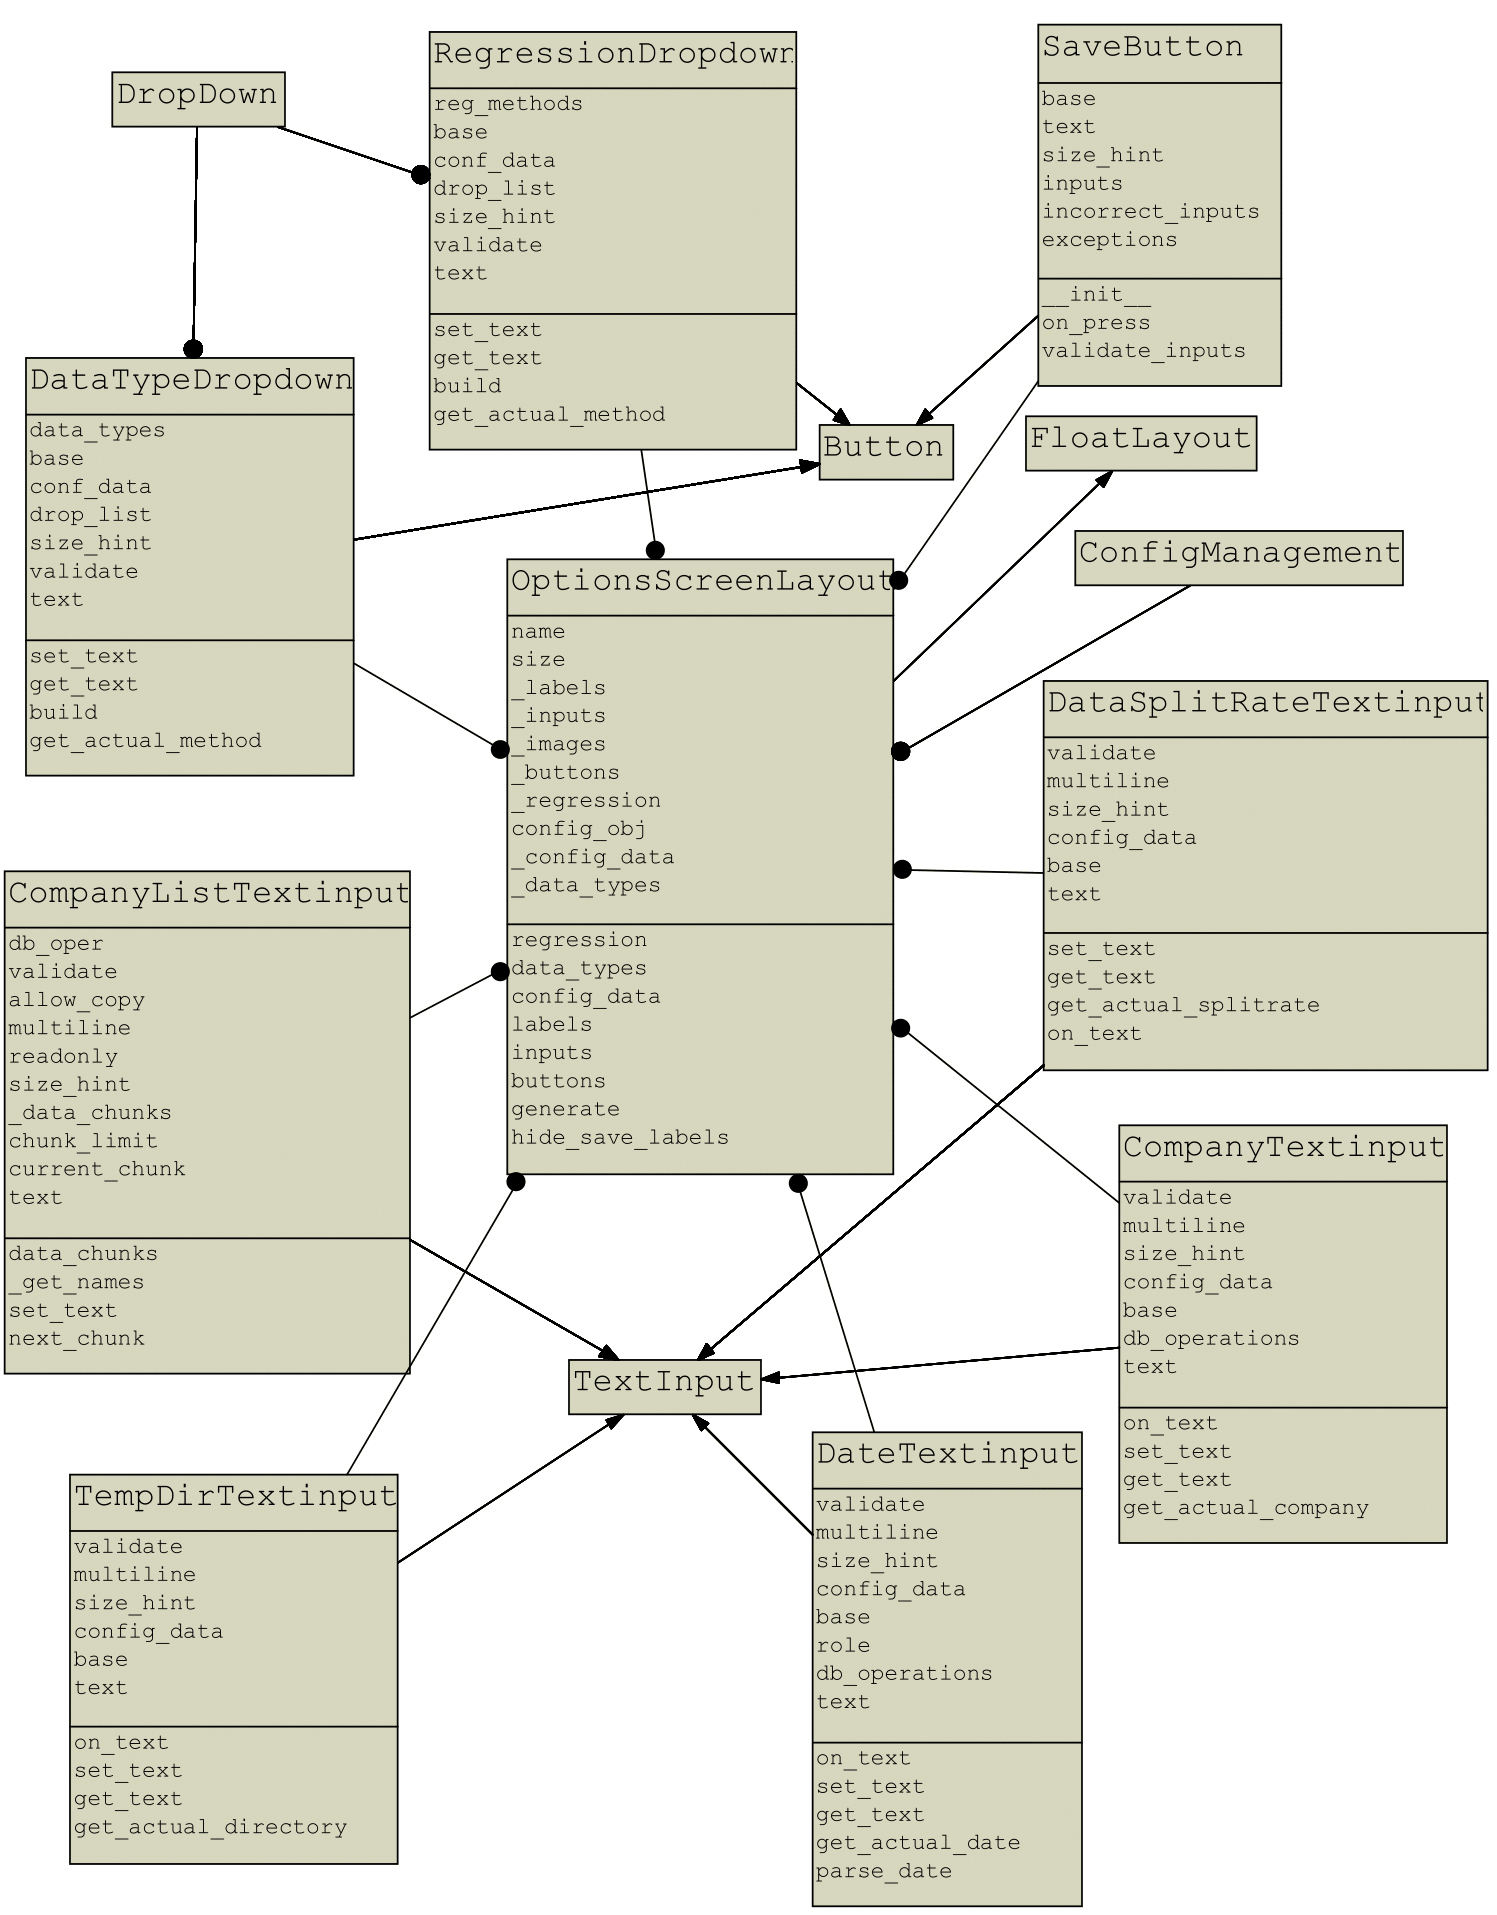
\includegraphics[scale=0.3]{pictures/uml_save.png}
\caption{Diagram UML: zapis parametrów w oknie opcji}
\label{fig:uml_zapis}
\end{figure}

\newpage

Podstawową klasą jest \textit{OptionsScreenLayout}, która dziedziczy po klasie \textit{FloatLayout} należącej do biblioteki \textit{Kivy}, 
a także implementuje klasy odpowiedzialne za zarządzenie konfiguracją (\textit{ConfigManagement}) oraz za przycisk zapisu konfiguracji (\textit{SaveButton}.)\\

Pozostałe klasy, w zależności od przeznaczenia, dziedziczą po pochodzących z pakietu \textit{Kivy} klasach \textit{TextInput} praz \textit{Button}.
Dwie klasy odpowiedzialne za implementację list rozwijanych dodatkowo implementują klasę \textit{DropDown}.\\

\subsection{Pobieranie danych giełdowych}
Kolejną funkcją aplikacji przedstawioną na schemacie UML jest mechanizm pobierania danych giełdowych.\\
\begin{figure}[ht]
\centering
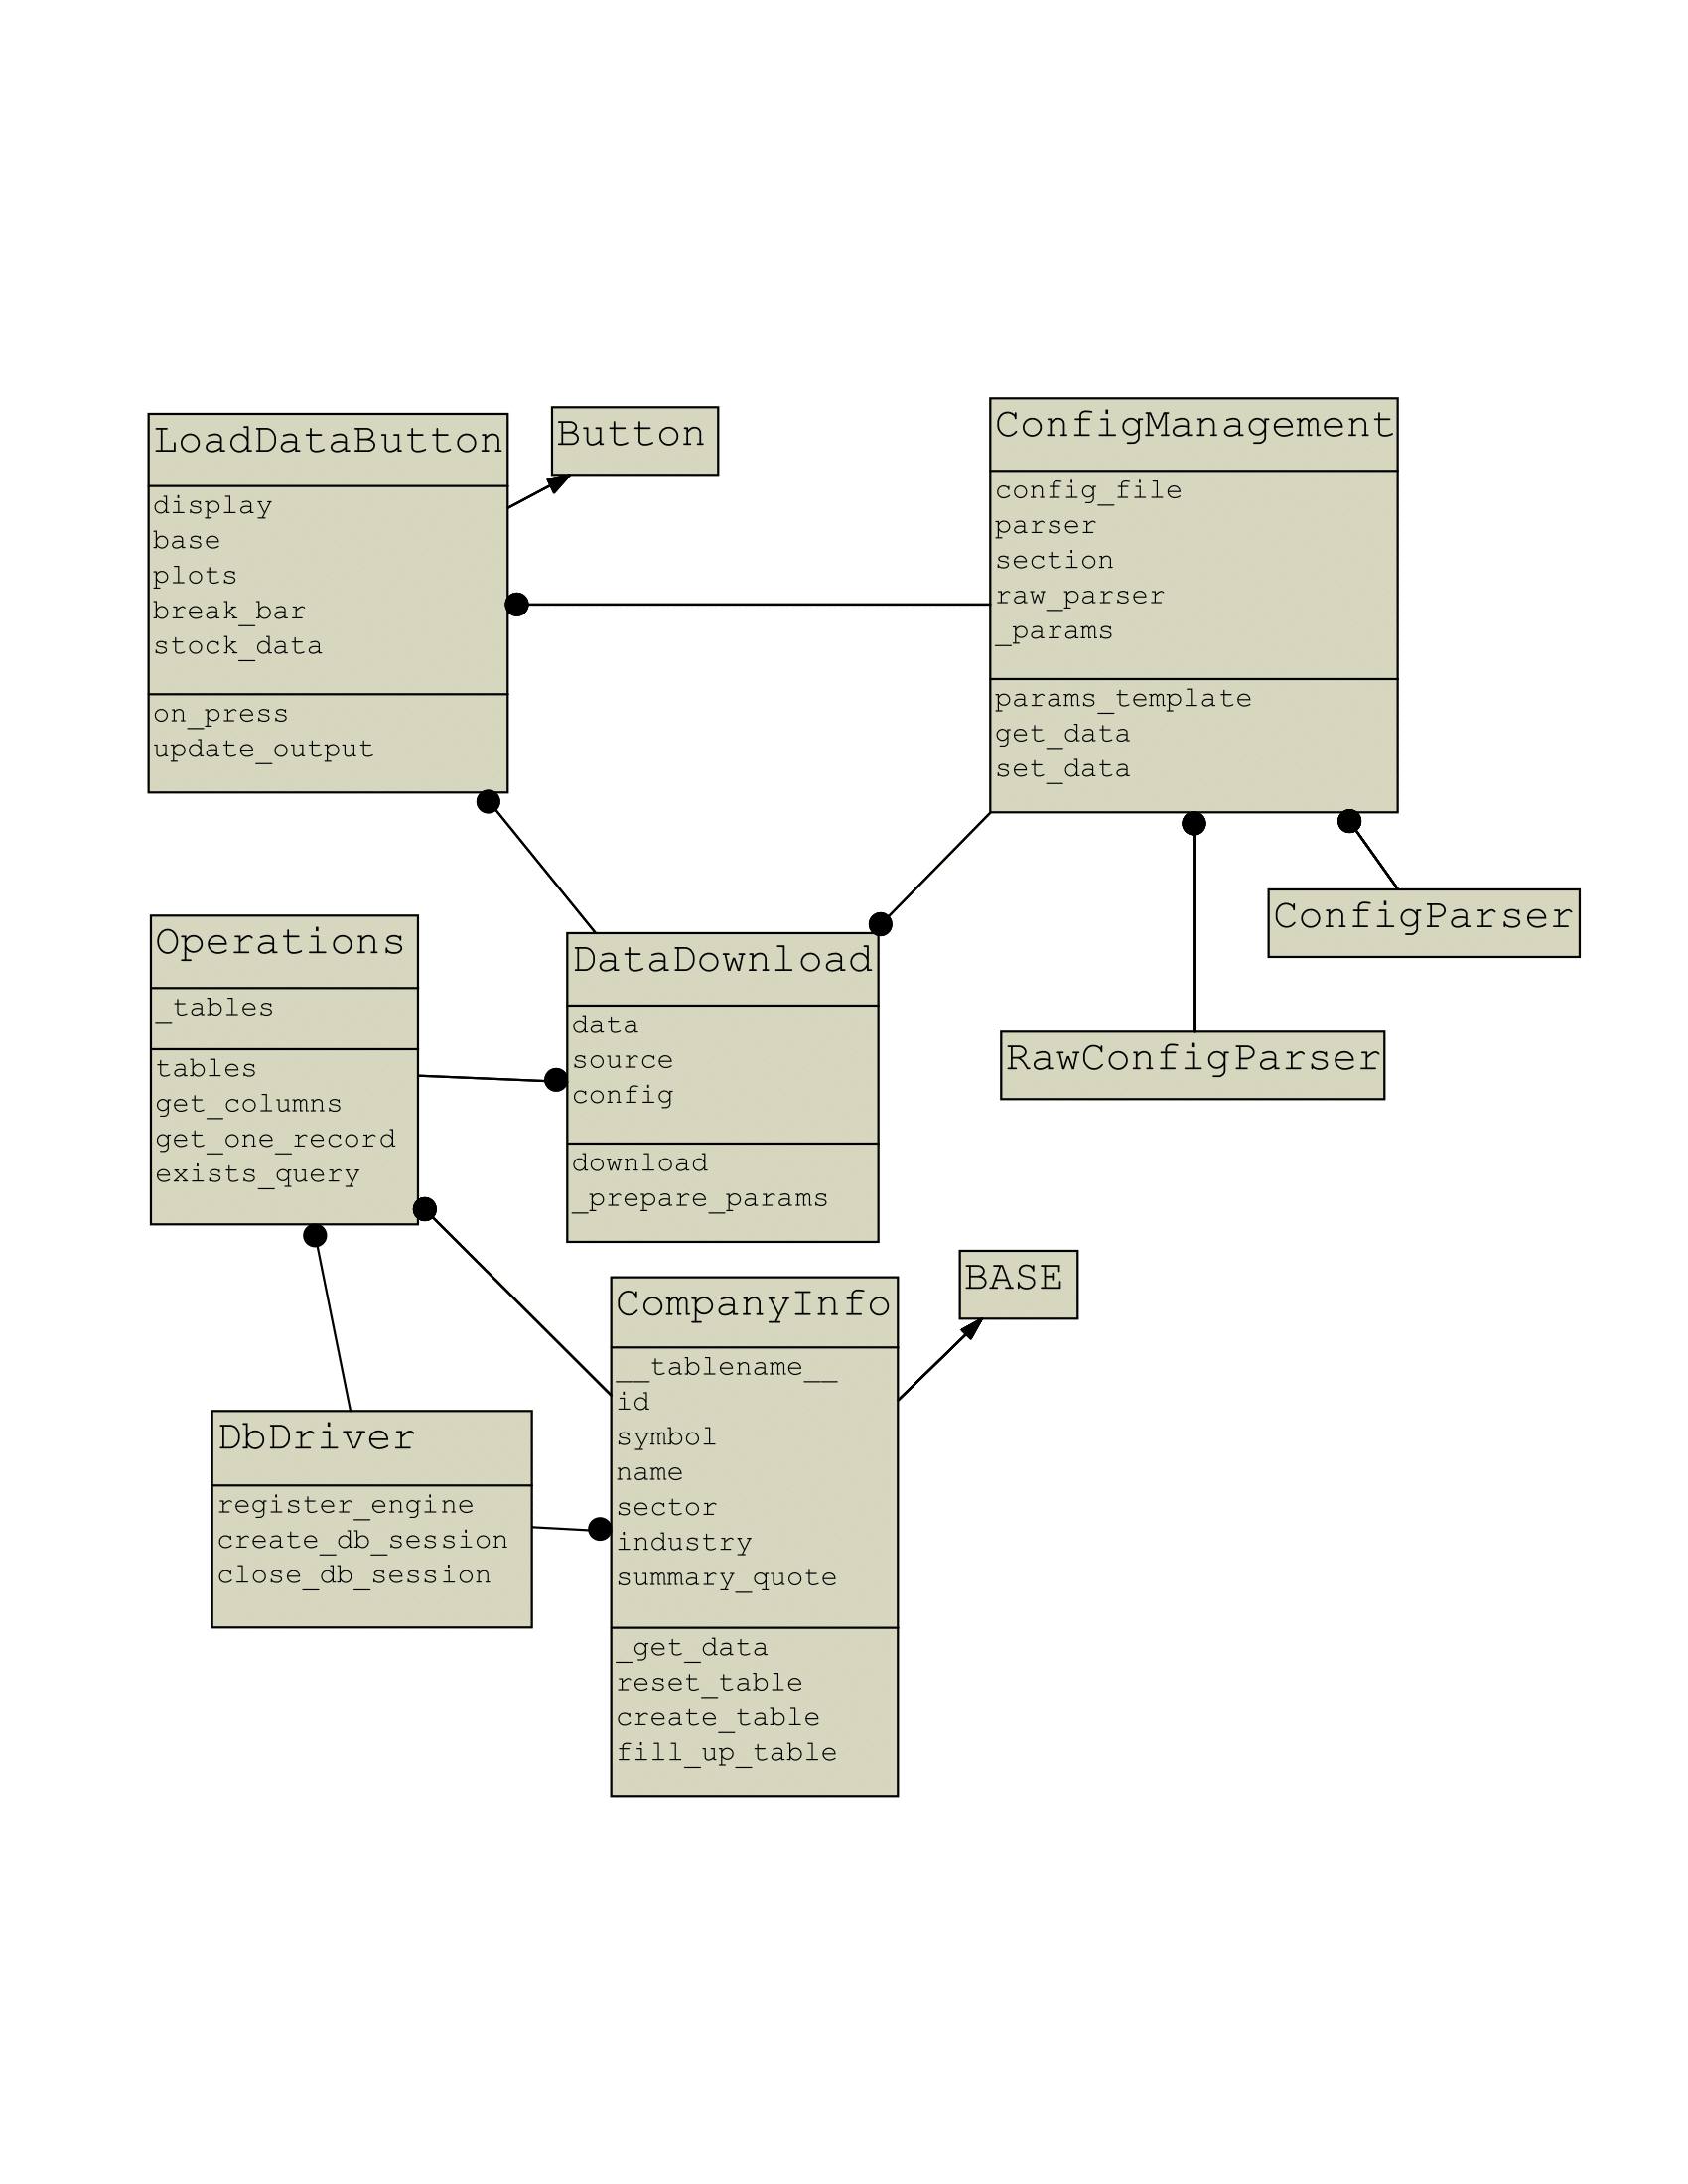
\includegraphics[scale=0.4]{pictures/uml_load_data.png}
\caption{Diagram UML: pobierane danych giełdowych}
\label{fig:uml_pobieranie}
\end{figure}

Przycisk odpowiedzialny za akcję, \textit{LoadDataButton}, dziedziczy po klasie \textit{Button} biblioteki \textit{Kivy}, oraz implementuje klasy zarządzania konfiguracją oraz pobierania danch (\textit{DataDownload}).
Klasa odpowiadająca za pobieranie danych implementuje natomiast bazodanową klasę \textit{Operations}, która wraz z \textit{CompanyInfo} oraz \textit{DbDriver} umożliwiają dostęp do bazy danych nazw i znaczników giełdowych firm.\\

\newpage

\subsection{Analiza regresji}
Ostatnią przedstawioną funkcją aplikacji jest przeprowadzanie analizy regresji.\\
\begin{figure}[ht]
\centering
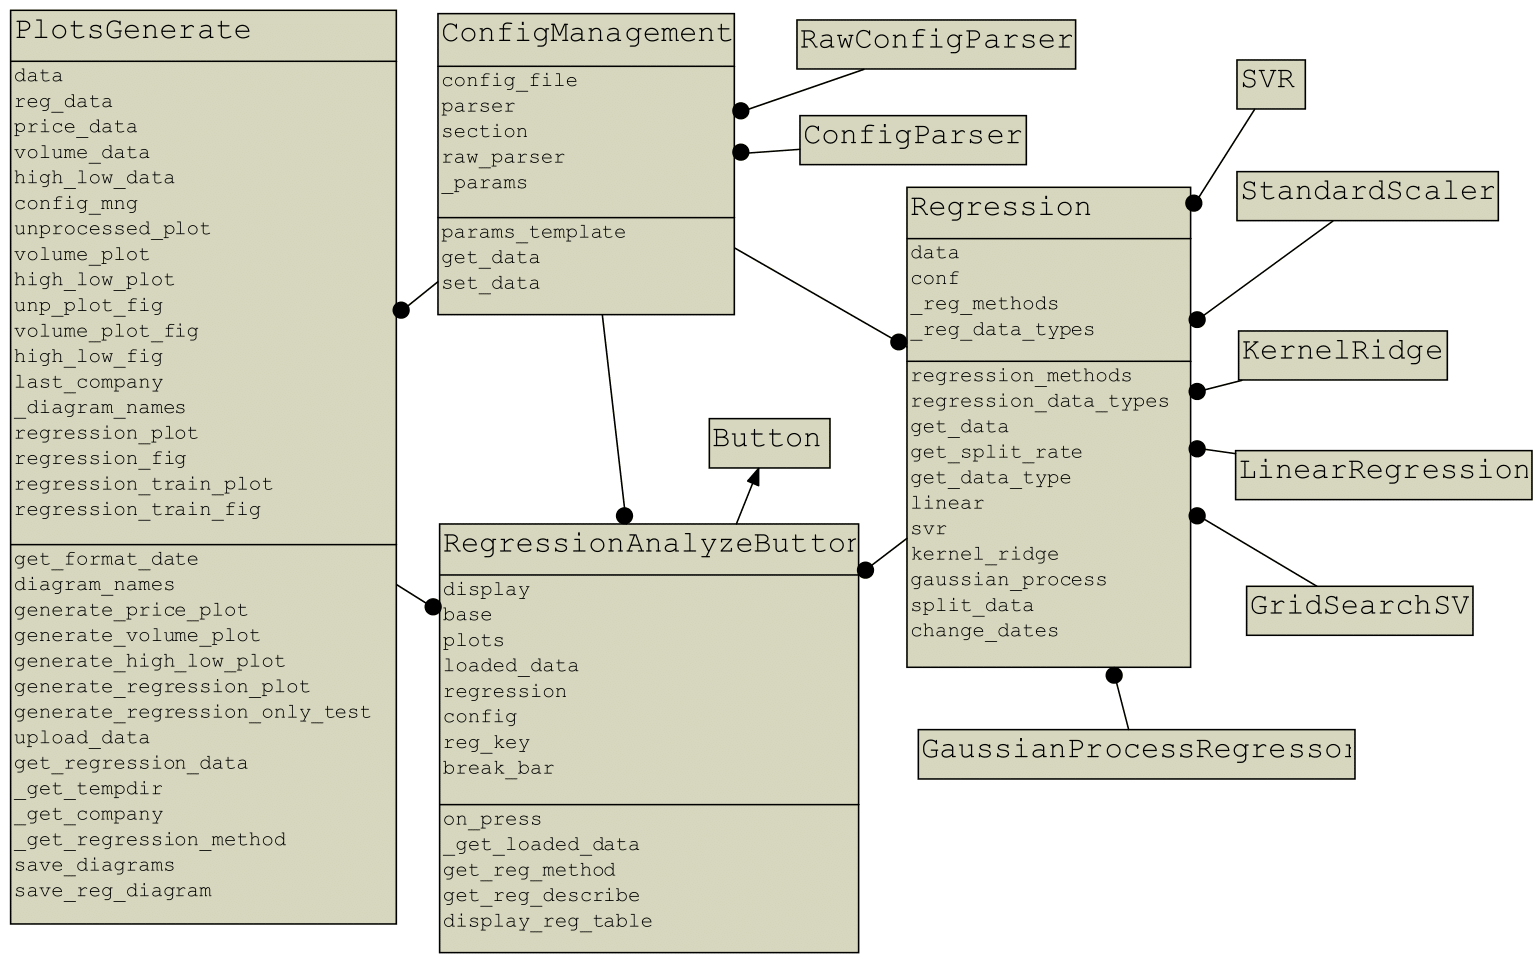
\includegraphics[scale=0.5]{pictures/uml_regression.png}
\caption{Diagram UML: analiza regresji}
\label{fig:uml_reg}
\end{figure}

Przycisk \textit{RegressionAnalyzeButton} implementuje zarówno klasy \textit{PlotsGenerate}, \textit{ConfigManagement} oraz \textit{Regression}.
Klasa \textit{Regression} natomiast, odpowiedzialna za przeprowadzenie właściwej analizy i zwrócenie wyników, implementuje szereg klas pochodzących z pakietu \textit{Scikit-learn}.\\